Nyní je tedy na čase připravit návrh řešení aplikace, která by zajistila správu modulárních dokumentů, jejich generování/publikaci. Nesmíme zapomenout
na důležité funkcionality, které jsme si stanovili v první části této kapitoly. Jedná se hlavně o správu uživatelů, možnost tvořit revize a celkově
verzovat jednotlivé části textu. Dále nesmíme zapomenout na možnost rozšíření aplikace.

\section{Užitelská sekce}

V uživatelské sekci bude hlavní důraz kladen na správu uživatelů, zde také musíme myslet na ochranu jejich osobních udajů a díky GDPR také na
možnost jejich anonymizace.

\subsection{GDPR}

Uživatele se člověk stává už pouhým otevřením naší aplikace, tento uživatel je nyní v roli hosta, který nemá žádné právo, poté má pouze 2 možnosti, buď se
přihlásí, nebo se registruje jako nový uživatel s právy. Po registraci následuje nutnost potvrdit uživatelský účet jako standardní účet.
Uživatel, stále v roli host, se nyní může přihlásit do aplikace, kde disponuje základními právy, jakými jsou spravování vlastních repozitářů a dokumentů,
či sdílení svých prací s ostatními uživateli se standardními právy. Také zde existuje administrátorská role, která má vyšší než standardní práva,
a to hlavně možnost kontrolovat ostatní uživatele.

O uživatelých si potřebujeme z osobních údajů pamatovat pouze e-mail a uživatelské jméno, které je unikátní pro každého uživatele. Dále si uchováváme
informace o datu založení, poslední změny a smazání uživatele. Dále si pamatujeme role, které uživatel má přiřazené. Role, krom našich základních čtyř
(host, standardní, administrátor, super administrátor), mohou být tvořeny administrátory, kteří je pak mohou přiřadit všem ostatním uživatelům. Podpoření
anonymizace bude založeno na změně uživatelského jména a emailu na sled náhodných znaků, ze kterých nebude patrný původní obsah, tzv. \textit{hash}. Každý z
uživatelů bude mít možnost smazat svůj účet, nebo si jej plně anonymizovat.

Za data, která užvatelé napíší již v rámci dokumentů neneseme odpovědnost, ovšem v případě smluv, či jiných například úředních dokumentů by bylo dobré
zajistit možnost jejich vyplnění až při vystavení dokumentu, aby pak tedy nemuseli být v aplikaci vůbec uloženy.
\todo{Question: Dopsat možnosti parametrizace dat, možná to napsat do analýzy, nebo ještě lépe, konzultovat}

% this might be used, but not now
% \begin{center}
%     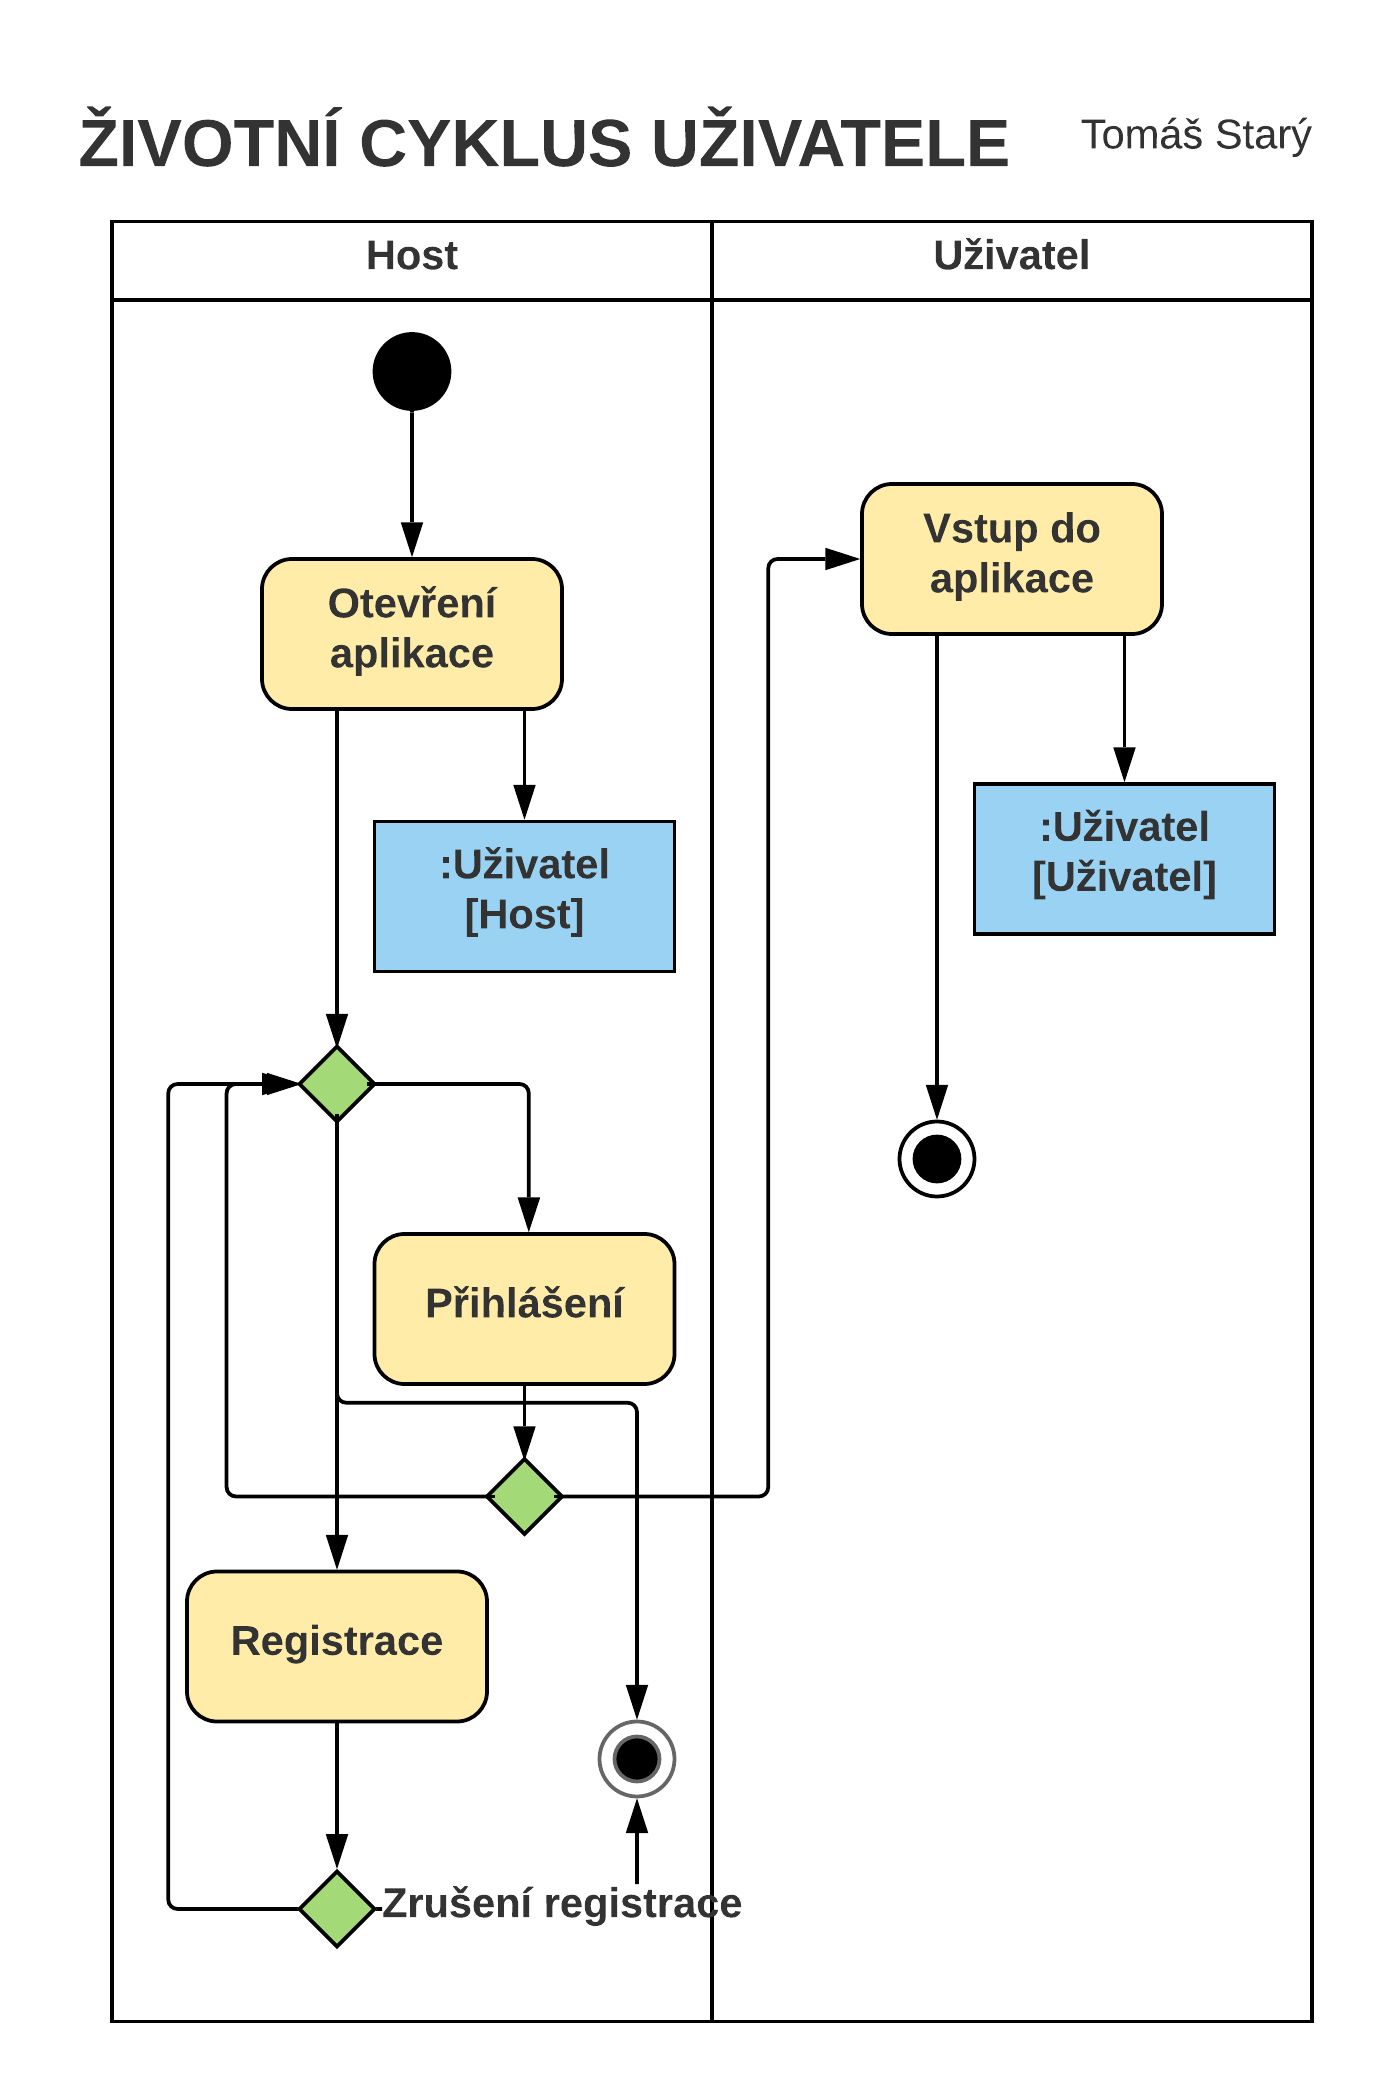
\includegraphics[width=8cm]{lifecycle.png}
% \end{center}